\subsection{Đề 2}
\Opensolutionfile{ans}[ans/ans-2-B16-De2]
\caulc
\begin{ex}%[Nguyễn Tuấn, dự án sáng tác đề 12 theo chủ đề]%[2H5H2-7]
	Cho hai mặt phẳng $(P_1)\colon A_1x+B_1y+C_1z+D_1=0$ $(A_1^2+B_1^2+C_1^2\ne 0)$ và \break $(P_2) \colon A_2x+B_2y+C_2z+D_2=0$ $(A_2^2+B_2^2+C_2^2\ne 0)$. Gọi $\varphi$ là góc giữa hai mặt phẳng $(P_1)$ và $(P_2)$. Hãy chọn khẳng định đúng?
	\choice
	{$\cos \varphi =\dfrac{\left|A_1A_2+B_1B_2+C_1C_2\right|}{(A_1^2+B_1^2+C_1^2)\cdot (A_2^2+B_2^2+C_2^2)}$}
	{\True $\cos \varphi =\dfrac{\left|A_1A_2+B_1B_2+C_1C_2\right|}{\sqrt{A_1^2+B_1^2+C_1^2}\cdot \sqrt{A_2^2+B_2^2+C_2^2}}$}
	{$\cos \varphi =\dfrac{A_1A_2+B_1B_2+C_1C_2}{(A_1^2+B_1^2+C_1^2)\cdot(A_2^2+B_2^2+C_2^2)}$}
	{$\cos \varphi =\dfrac{A_1A_2+B_1B_2+C_1C_2}{\sqrt{A_1^2+B_1^2+C_1^2}\cdot\sqrt{A_2^2+B_2^2+C_2^2}}$}
	\loigiai
	{
		Gọi $\overrightarrow{n}_1$ và $\overrightarrow{n}_2$ lần lượt là véc-tơ pháp tuyến của mặt phẳng $(P_1)$ và $(P_2)$.\\
		Ta có $\cos \varphi = \dfrac{\left|\overrightarrow{n}_1\cdot \overrightarrow{n}_2\right|}{\left|\overrightarrow{n}_1\right|\cdot \left|\overrightarrow{n}_2\right|}=\dfrac{\left|A_1A_2+B_1B_2+C_1C_2\right|}{\sqrt{A_1^2+B_1^2+C_1^2}\cdot\sqrt{A_2^2+B_2^2+C_2^2}}$
	}
\end{ex}
\begin{ex}%[Nguyễn Tuấn, dự án sáng tác đề 12 theo chủ đề]%[2H5H2-7]
	Trong không gian $Oxyz$ cho hai mặt phẳng $(P)\colon 2x - y-2z-9=0$,\break $(Q)\colon  x - y - 6=0$. Góc giữa hai mặt phẳng  $(P)$, $(Q)$ bằng
	\choice
	{$90^\circ$}
	{$30^\circ$}
	{\True $45^\circ$}
	{$60^\circ$}
	\loigiai
	{
		$(P)\colon 2x - y-2z-9=0$ có $1$ véc-tơ pháp tuyến là $\overrightarrow{n}_1 = (2;-1;-2)$.\\
		$(Q)\colon  x - y - 6=0$ có $1$ véc-tơ pháp tuyến là $\overrightarrow{n}_2 = (1;-1;0)$.\\
		$\cos \left(\left( P \right),\left( Q \right)\right) = \dfrac{\left|\overrightarrow{n}_1\cdot \overrightarrow{n}_2\right|}{\left|\overrightarrow{n}_1\right|\cdot \left|\overrightarrow{n}_2\right|} $
		$= \dfrac{\left|2\cdot 1 + \left(- 1\right)\left(- 1\right) + 0\right|}{\sqrt{2^2 + 1^2 + 2^2}\cdot \sqrt{1^2+ 1^2 + 0}}= \dfrac{1}{\sqrt{2}} \Rightarrow \left(\left( P \right),\left( Q \right)\right) = 45^\circ$.
	}
\end{ex}
\begin{ex}%[Nguyễn Tuấn, dự án sáng tác đề 12 theo chủ đề]%[2H5H2-7]
	Tính số đo góc giữa mặt phẳng $(P)\colon x + z - 4 = 0$ và mặt phẳng $(Oxy)$.
	\choice
	{$30^\circ$}
	{$90^\circ$}
	{$60^\circ$}
	{\True $45^\circ$}
	\loigiai{
		Ta có véc-tơ pháp tuyến của hai mặt phẳng là $\overrightarrow{n}_{(P)} = (1; 0; 1)$, $\overrightarrow{n}_{(Oxy)} = \overrightarrow{k} = (0; 0; 1)$.\\
		Khi đó $\left|\overrightarrow{n}_{(P)}\right| = \sqrt{2}$; $\left|\overrightarrow{n}_{(Oxy)}\right| = 1$.\\
		Ta có $$\cos ((P),(Oxy))=|\cos \left(\overrightarrow{n}_{(P)}, \overrightarrow{n}_{(Oxy)}\right)| = \dfrac{\left|\overrightarrow{n}_{(P)} \cdot \overrightarrow{n}_{(Oxy)}\right|}{\left|\overrightarrow{n}_{(P)}\right| \cdot \left|\overrightarrow{n}_{(Oxy)}\right|} = \dfrac{1}{\sqrt{2}} = \dfrac{\sqrt{2}}{2}.$$
		Suy ra góc giữa hai mặt phẳng đã cho bằng $45^\circ$.
	}
\end{ex}
\begin{ex}%[Nguyễn Tuấn, dự án sáng tác đề 12 theo chủ đề]%[2H5H2-7]
	Trong không gian $Oxyz$, cho hai mặt phẳng $(P)\colon x-y-6=0$ và $(Q)$. Biết rằng điểm $H(2;-1;-2)$ là hình chiếu vuông góc của gốc tọa độ $O(0;0;0)$ xuống mặt phẳng $(Q)$. Số đo góc giữa hai mặt phẳng $(P)$ và mặt phẳng $(Q)$ bằng
	\choice
	{\True $45^\circ$}
	{$60^\circ$}
	{$30^\circ$}
	{$90^\circ$}
	\loigiai{
		Ta có $\overrightarrow{OH}=\left(2;-1;-2\right)$ là véc-tơ pháp tuyến của $(Q)$, $\overrightarrow{n}=(1;-1;0)$ là véc-tơ pháp tuyến của $(P)$.\\
		Gọi $\alpha$ là góc giữa hai mặt phẳng $(P)$ và $(Q)$, ta có
		$$\cos\alpha =\dfrac{\left|\overrightarrow{OH}\cdot\overrightarrow{n}\right|}{\left|\overrightarrow{OH}\right|\cdot\left|\overrightarrow{n}\right|}=\dfrac{|2+1|}{3\sqrt{2}}=\dfrac{1}{\sqrt{2}}\Rightarrow \alpha =45^\circ.$$
	}
\end{ex}
\begin{ex}%[Nguyễn Tuấn, dự án sáng tác đề 12 theo chủ đề]%[2H5H2-7]
	Trong không gian với hệ trục tọa độ $Oxyz$, cho mặt phẳng $(P) \colon x-y+2z+1=0$ và đường thẳng $d\colon \dfrac{x-1}{1}=\dfrac{y}{2}=\dfrac{z+1}{-1}$. Tính góc giữa đường thẳng $d$ và mặt phẳng $(P)$.
	\choice
	{$60^{\circ} $}
	{$120^{\circ} $}
	{$150^{\circ} $}
	{\True $30^{\circ} $}
	\loigiai{
		Ta có $\overrightarrow{u}_{d}=(1;2;-1)$ và $\overrightarrow{n}_{(P)}=(1;-1;2)$.\\
		Do đó $\sin (d,(P))=|\cos(\overrightarrow{u}_d,\overrightarrow{n}_{(P)})|=\dfrac{|1-2-2|}{\sqrt{6} \cdot \sqrt{6}}=\dfrac{1}{2}$, suy ra góc giữa đường thẳng $d$ và mặt phẳng $(P)$ bằng $30^{\circ}$.
	}
\end{ex}
\begin{ex}%[Nguyễn Tuấn, dự án sáng tác đề 12 theo chủ đề]%[2H5H2-7]
	Trong không gian với hệ tọa độ $Oxyz$, cho đường thẳng $d: \heva{&x=5+t\\ &y=-2+t\\ &z=4+\sqrt{2}t},\, (t\in\mathbb{R})$ và mặt phẳng $(P): x-y+\sqrt{2}z-7=0$. Hãy xác định góc giữa đường thẳng $d$ và mặt phẳng $(P)$.
	\choice
	{$90^\circ$}
	{$45^\circ$}
	{\True $30^\circ$}
	{$60^\circ$}
	\loigiai{
		Đường thẳng $d$ có véc-tơ chỉ phương $\overrightarrow{u}=(1;1;\sqrt{2})$.\\
		Mặt phẳng $(P)$ có véc-tơ pháp tuyến $\overrightarrow{n}=(1;-1;\sqrt{2})$.\\
		Gọi $\varphi$ là góc giữa đường thẳng và mặt phẳng, khi đó ta có
		$$\sin\varphi=\dfrac{\left|\overrightarrow{u}\cdot\overrightarrow{n}\right|}{|\overrightarrow{u}|\cdot|\overrightarrow{n}|}=\dfrac{|1\cdot1+1\cdot(-1)+\sqrt{2}\cdot\sqrt{2}|}{\sqrt{1^2+1^2+(\sqrt{2})^2}\cdot\sqrt{1^2+(-1)^2+(\sqrt{2})^2}}=\dfrac{1}{2}.$$
		Từ đó suy ra $\varphi=30^\circ$.
	}
\end{ex}
\begin{ex}%[Nguyễn Tuấn, dự án sáng tác đề 12 theo chủ đề]%[2H5H2-7]
	Trong không gian $Oxyz$, cho hai đường thẳng $\Delta_1\colon \dfrac{x-1}{-2}=\dfrac{y+2}{1}=\dfrac{z-3}{2}$ và $\Delta_2\colon \dfrac{x+3}{1}=\dfrac{y-1}{1}=\dfrac{z+2}{-4}$. Góc giữa hai đường thẳng $\Delta_1$ và $\Delta_2$ bằng
	\choice
	{$30^\circ$}
	{\True $45^\circ$}
	{$60^\circ$}
	{$135^\circ$}
	\loigiai{
		Véc-tơ chỉ phương của $\Delta_1$ và $\Delta_2$	 lần lượt là $\overrightarrow{u}_1=(-2;1;2)$ và $\overrightarrow{u}_2=(1;1;-4)$. Khi đó 
		\[ \cos\left(\Delta_1,\Delta_2\right)=\dfrac{\left|\overrightarrow{u}_1\cdot\overrightarrow{u}_2\right|}{\left|\overrightarrow{u}_1\right|\cdot\left|\overrightarrow{u}_2\right|}=\dfrac{\left|(-2)\cdot 1+1\cdot 1+2\cdot(-4)\right|}{\sqrt{(-2)^2+1^2+2^2}\cdot\sqrt{1^2+1^2+(-4)^2}}=\dfrac{\sqrt{2}}{2}. \]
		Do đó góc giữa hai đường thẳng $\Delta_1$ và $\Delta_2$ là $45^\circ$.
	}
\end{ex}
\begin{ex}%[Nguyễn Tuấn, dự án sáng tác đề 12 theo chủ đề]%[2H5H2-7]
	Trong không gian với hệ tọa độ $Oxyz$, cho ba điểm $A(1; 2; 3)$, $B(2; 1; 5)$, $C(2; 4; 2)$. Tính góc giữa hai đường thẳng $AB$ và $AC$.
	\choice
	{\True $60^{\circ}$}
	{$150^{\circ}$}
	{$30^{\circ}$}
	{$120^{\circ}$}
	\loigiai{
		Ta có $\overrightarrow{AB}=(1;-1;2)$, $\overrightarrow{AC}=(1; 2;-1)$ nên $$\cos(AB,AC)=\left|\cos\left(\overrightarrow{AB},\overrightarrow{AC}\right)\right|=\dfrac{\left|\overrightarrow{AB}\cdot\overrightarrow{AC}\right|}{\left|\overrightarrow{AB}\right|\cdot\left|\overrightarrow{AC}\right|}=\dfrac{|1-2-2|}{\sqrt{6}\cdot \sqrt{6}}=\dfrac{1}{2} \Rightarrow \left(AB,AC\right)=60^\circ.$$}
\end{ex}
\begin{ex}%[Nguyễn Tuấn, dự án sáng tác đề 12 theo chủ đề]%[2H5H2-7]
	Trong không gian với hệ tọa độ $Oxyz$ cho mặt phẳng $(P)\colon 3x+4y+5z+8=0$ và đường thẳng $d$ là giao tuyến của hai mặt phẳng $(\alpha)\colon x-2y+1=0$ và $(\beta)\colon x-2z-3=0$. Tính góc $\varphi$ giữa $d$ và $(P)$
	\choice
	{$\varphi=30^{\circ}$}
	{$\varphi=45^{\circ}$}
	{\True $\varphi=60^{\circ}$}
	{$\varphi=90^{\circ}$}
	\loigiai{
		Các véc-tơ pháp tuyến của các mặt phẳng $(P)$, $(\alpha)$, $(\beta)$ lần lượt là $\overrightarrow{n}_1=(3;4;5)$, $\overrightarrow{n}_2=(1;-2;0)$, $\overrightarrow{n_3}=(1;0;-2)$.\\
		Ta có  $\overrightarrow{u}=\left[\overrightarrow{n}_2,\overrightarrow{n_3}\right]=(4;2;2)$ là một véc-tơ chỉ phương của đường thẳng $d$. Do đó
		$$\sin\varphi=\dfrac{\left|\overrightarrow{u}\cdot\overrightarrow{n}_1\right|}{\left|\overrightarrow{u}\right|\cdot \left|\overrightarrow{n}_1\right|}=\dfrac{|3\cdot 4+4\cdot 2+5\cdot 2|}{\sqrt{3^2+4^2+5^2}\cdot\sqrt{4^2+2^2+2^2}}=\dfrac{\sqrt{3}}{2}\Rightarrow\varphi=60^{^{\circ}}.$$}
\end{ex}
\begin{ex}%[Nguyễn Tuấn, dự án sáng tác đề 12 theo chủ đề]%[2H5H2-7]
	Trong không gian $Oxyz$  cho $2$ đường thẳng $d_1\colon \dfrac{x+1}{2} = \dfrac{y-1}{-m} =\dfrac{z-2}{-3}$,  $d_2\colon \dfrac{x-3}{1} = \dfrac{y}{1} =\dfrac{z-1}{1}$. Tìm tất cả giá trị thực của $m$ để $d_1$ vuông góc với $d_2$
	\choice
	{\True $m=-1$}
	{$m=1$}
	{$m=-5$}
	{$m=5$}
	\loigiai{
		Véc-tơ chỉ phương của $d_1$, $d_2$ lần lượt là $\overrightarrow{u}_1 = (2;-m;-3)$ và $\overrightarrow{u}_2 = (1;1;1)$. \\ Để $d_1 \perp d_2$ thì $\overrightarrow{u}_1  \cdot \overrightarrow{u}_2 = 0 \Leftrightarrow 2-m-3 = 0 \Leftrightarrow m =-1 .$ 
	}
\end{ex}
\begin{ex}%[Nguyễn Tuấn, dự án sáng tác đề 12 theo chủ đề]%[2H5H2-7]
	Trong không gian $Oxyz$ cho điểm $A(0;2;2)$. Góc giữa đường thẳng $OA$ và trục $Oy$ bằng
	\choice
	{$60^{\circ}$}
	{$30^{\circ}$}
	{$90^{\circ}$}
	{\True $45^{\circ}$}
	\loigiai{
		Đường thẳng $OA$ có một véc-tơ chỉ phương là $\overrightarrow{OA}=(0;2;2)$, trục $Oy$ có một véc-tơ chỉ phương là $\overrightarrow{j}=(0;1;0)$.\\
		Ta có $\cos \left(\overrightarrow{OA},\overrightarrow{j}\right) = \dfrac{\overrightarrow{OA} \cdot \overrightarrow{j}}{\left|\overrightarrow{OA}\right| \cdot \left|\overrightarrow{j}\right| }= \dfrac{2}{2\sqrt{2}} = \dfrac{\sqrt{2}}{2} \Rightarrow \left(\overrightarrow{OA},\overrightarrow{j}\right) =45^{\circ}$.\\
		Suy ra góc giữa đường thẳng $OA$ và trục $Oy$ là $45^{\circ}$.
	}
\end{ex}
\begin{ex}%[Nguyễn Tuấn, dự án sáng tác đề 12 theo chủ đề]%[2H5V2-7]
	Trong không gian $Oxyz$, hai đường thẳng $d_1\colon\dfrac{x-2}{1}=\dfrac{y+1}{\sqrt{2}}=\dfrac{z-3}{1}$ và $d_2\colon\dfrac{x+5}{1}=\dfrac{y+3}{\sqrt{2}}=\dfrac{z-5}{m}$ tạo với nhau góc $60^\circ$, giá trị của tham số $m$ bằng
	\choice
	{\True $ m=-1 $}
	{$ m=\dfrac{\sqrt{3}}{2} $}
	{$ m=\dfrac{1}{2} $}
	{$ m=1 $}
	\loigiai{
		Ta có véc-tơ chỉ phương của hai đường thẳng $d_1$, $d_2$ lần lượt là $\overrightarrow{u}_1=\left(1;\sqrt{2};1\right) $ và $\overrightarrow{u}_2=\left( 1;\sqrt{2};m\right) $.\\ 
		Theo công thức tính góc tạo bởi hai đường thẳng thì $\cos \varphi =\dfrac{\left|  \overrightarrow{u}_1\cdot\overrightarrow{u}_2\right| }{|\overrightarrow{u}_1|\cdot |\overrightarrow{u}_2|}$ với $\varphi=(d_1,d_2)$.\\
		Từ giả thiết suy ra
		\begin{eqnarray*}
			&&\dfrac{1}{2}=\dfrac{|3+m|}{2\sqrt{m^2+3}}\\
			&\Leftrightarrow &\sqrt{m^2+3}=|3+m|\Leftrightarrow m^2+3=m^2+6m+9\\
			&\Leftrightarrow &m=-1.
		\end{eqnarray*}
	}  
\end{ex}
\Closesolutionfile{ans}
\indapan{6}{ans/ans-2-B16-De2}
\cauds
\Opensolutionfile{ans}[ans/ans-2-B16-De2-DS]
\begin{ex}%[Nguyễn Tuấn, dự án sáng tác đề 12 theo chủ đề]%[2H5H2-7]
	Trong không gian với hệ tọa độ $Oxyz$, cho mặt phẳng $(P)\colon x-y+2z+1=0$ và đường thẳng $d\colon\dfrac{x-1}{1}=\dfrac{y}{2}=\dfrac{z+1}{-1}$. Xác định tính đúng, sai của mỗi mệnh đề sau
	\choiceTF
	{\True Một véc-tơ chỉ phương của $d$ là $(1;2;-1)$}
	{Một véc-tơ pháp tuyến của $(P)$ là $(-1;2;1)$.}
	{\True $\left(d,(P)\right)=30^{\circ}$}
	{\True Nếu điểm $M$ thuộc $d$ có hoành độ bằng $2$ thì $\mathrm{d}(M,(P))=\dfrac{\sqrt{6}}{2}$}
	\loigiai{
		\begin{itemchoice}
			\itemch 	Ta có $\overrightarrow{n}_{(P)}=(1;-1; 2)$
			\itemch Ta có $\overrightarrow{u}_d=(1; 2;-1)$.
			\itemch Ta có $\sin\left(d,(P)\right)=\dfrac{\left|\overrightarrow{n}_{(P)}\cdot\overrightarrow{u}_d\right|}{\left|\overrightarrow{n}_{(P)}\right|\cdot\left|\overrightarrow{u}_d\right|} =\dfrac{|1-2-2|}{\sqrt{6}\cdot\sqrt{6}}=\dfrac{1}{2}\Rightarrow \left(d,(P)\right)=30^{\circ}$.
			\itemch Điểm $M$ thuộc $d$ mà có hoành độ bằng $2$ thì $M(2;2;-2)$. Vậy 
			$$\mathrm{d}(M,(P))=\dfrac{|2-2+2\cdot (-2)+1|}{\sqrt{1^2+(-1)^2+2^2}}=\dfrac{\sqrt{6}}{2}.$$
		\end{itemchoice}
	}
\end{ex}
\begin{ex}%[Nguyễn Tuấn, dự án sáng tác đề 12 theo chủ đề]%[2H5H2-7]
	Cho đường thẳng $
	\Delta\colon \dfrac{x}{2}=\dfrac{y}{-1}=\dfrac{z}{2}$.
	\choiceTF
	{\True 	Đường thẳng $\Delta$ có $1$ véc-tơ chỉ phương là $\overrightarrow{u}_{\Delta}=(2;-1;2)$}
	{Cosin của góc giữa đường thẳng $\Delta$ và trục $Ox$ bằng $\dfrac{\sqrt{5}}{5}$}
	{\True Cosin của góc giữa đường thẳng $\Delta$ và trục $Oy$ bằng $\dfrac{\sqrt{5}}{5}$}
	{\True Cosin của góc giữa đường thẳng $\Delta$ và trục $Oz$ bằng $\dfrac{2\sqrt{5}}{5}$}
	\loigiai{
		\begin{itemchoice}
			\itemch Đúng. Đường thẳng $\Delta$ có véc-tơ chỉ phương là $\overrightarrow{u}_{\Delta}=(2;-1;2)$.
			\itemch Sai. Trục $ Ox $	có véc-tơ chỉ phương là $\overrightarrow{u}_1=(1;0;0)$. Ta có
			\[\cos \left(\Delta, Ox\right)=\dfrac{|2 \cdot1+(-1)\cdot 0+2 \cdot 0|}{\sqrt{2^2+(-1)^2+2^2} \cdot \sqrt{1^2+0^2+0^2}}=\dfrac{2\sqrt{5}}{5},\]
			\itemch Đúng. Trục $ Oy $	có véc-tơ chỉ phương là $\overrightarrow{u}_2=(0;1;0)$. Ta có
			\[\cos \left(\Delta, Oy\right)=\dfrac{|2 \cdot0+(-1)\cdot 1+2 \cdot 0|}{\sqrt{2^2+(-1)^2+2^2} \cdot \sqrt{0^2+1^2+0^2}}=\dfrac{\sqrt{5}}{5},\]
			\itemch Đúng. Trục $ Oz $	có véc-tơ chỉ phương là $\overrightarrow{u}_3=(0;0;1)$. Ta có
				\[\cos \left(\Delta, Oz\right)=\dfrac{|2 \cdot 0+(-1)\cdot 0+2 \cdot 1|}{\sqrt{2^2+(-1)^2+2^2} \cdot \sqrt{0^2+0^2+1^2}}=\dfrac{2\sqrt{5}}{5}.\]
		\end{itemchoice}
	}
\end{ex}
\begin{ex}%[Nguyễn Tuấn, dự án sáng tác đề 12 theo chủ đề]%[2H5V2-7] 
	Trong không gian với hệ tọa độ $O x y z$, một cabin cáp treo xuất phát từ điểm $A(10 ; 3 ; 0)$ và chuyển động đều theo đường cáp có véc-tơ chỉ phương là $\overrightarrow{u}=(2 ;-2 ; 1)$ với tốc độ là 4,5 m/s (đơn vị trên mỗi trục tọa độ là mét) (Hình bên dưới).
	\definecolor{ecru}{rgb}{0.76, 0.7, 0.5}
	\definecolor{darkolivegreen}{rgb}{0.33, 0.42, 0.18}
	\definecolor{deepskyblue}{rgb}{0.0, 0.75, 1.0}
	\definecolor{antiquebrass}{rgb}{0.8, 0.58, 0.46}
	\definecolor{arsenic}{rgb}{0.23, 0.27, 0.29}
	\definecolor{ashgrey}{rgb}{0.7, 0.75, 0.71}\definecolor{alizarin}{rgb}{0.82, 0.1, 0.26}
	\begin{center}
		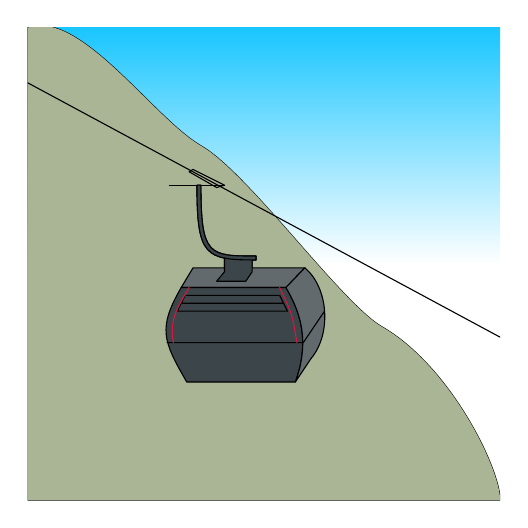
\begin{tikzpicture}[line join=round, line cap=round,scale=1,transform shape]
			\clip (-3,-3) rectangle (3,3);
			\fill[bottom color=white,top color=deepskyblue!90, middle color=white] (-3,-3) rectangle (3,3);
			\tikzset{dat/.pic={
					\def\N{ 
						(-3,3)
						..controls +(20:.7) and +(150:.7) ..(-.8,1.5)
						..controls +(-30:.7) and +(150:.6) ..(1.5,-.8)
						..controls +(-30:1) and +(90:.4) ..(3,-3)--(-3,-3)--cycle
						;
					}
					\draw[black]\N;
					\fill[darkolivegreen!50] \N;
			}}
			\tikzset{cap_treo/.pic={
					\def\X{ 
						(-.85,1)--(-.8,1)
						..controls +(-90:.9) and +(-180:.6) ..(-.1,0.1)--(-.1,.05)
						..controls +(-180:.65) and +(-90:.9) ..cycle
						(-.15,0.05)--(-.15,-.1)--(-.23,-.22)--(-.6,-.22)--(-.5,-.1)--(-.5,.08)
						;
					}
					%\fill[black] \X;
					\draw\X;
					\draw(-3,2.3)--(3.5,-1.2);
					\draw(-1.2,1)--(-.5,1);
					\draw(-.5,1)--(-.9,1.2)--(-.95,1.17)--(-.6,.97)--cycle;
					\draw[fill=arsenic!80](-.9,-.05)--(.52,-.05)--(.28,-.3)--(-1.05,-.3)--cycle;
					\def\M{ 
						(-.85,1)--(-.8,1)
						..controls +(-90:.9) and +(-180:.6) ..(-.1,0.1)--(-.1,.05)
						..controls +(-180:.65) and +(-90:.9) ..cycle
						(-.15,0.05)--(-.15,-.1)--(-.23,-.22)--(-.6,-.22)--(-.5,-.1)--(-.5,.08)
						;
					}
					\fill[arsenic] \M;
					\draw\M;
					\def\N{ 
						(-1.05,-.3)
						..controls +(-120:.6) and +(120:.6) ..(-.98,-1.5)--(.4,-1.5)
						..controls +(70:.6) and +(-60:.3) ..(.28,-.3)--cycle
						;
					}
					\fill[arsenic] \N;
					\draw\N;
					\def\P{ 
						(.4,-1.5)
						..controls +(70:.6) and +(-60:.3) ..(.28,-.3)--(.52,-.05)
						..controls +(-40:.4) and +(50:.4) ..(.6,-1.2)--cycle
						;
					}
					\fill[arsenic!80] \P;
					\draw\P;
					\draw (-1.23,-1)--(.5,-1)--(.77,-.6);
					\draw (-1.05,-.5)--(-1,-.4)--(.2,-.4)--(.25,-.5)--cycle
					(.25,-.5)--(.3,-.6)--(.3,-.6)--(-1.1,-.6)--(.-1.05,-.5)--cycle
					;
					\draw[alizarin](.42,-1)..controls +(100:.4) and +(-65:.4) ..(.2,-.3);
					\draw[alizarin](-1.15,-1)..controls +(100:.3) and +(-120:.3) ..(-.95,-.3);
			}}
			\path
			(0,0)pic[scale=1]{dat}(0,0)pic[scale=1]{cap_treo};
		\end{tikzpicture}
		\begin{tikzpicture}[scale=1, font=\footnotesize, line join=round,xscale=.2, line cap=round,>=stealth]
			\def\a{1/16} 
			\def\xmin{-3} \def\xmax{12}
			\def\ymin{-3} \def\ymax{3} 
			\coordinate (O) at (0,0);
			\coordinate (E) at (-10,-3);
			\coordinate (N) at ($(E)!.7!(O)$);
			\coordinate (P) at ($(E)!.2!(O)$);
			\coordinate (D) at ($(E)!.3!(O)$);
			\coordinate (A) at ($(N)+(3,0)$);
			\coordinate (B) at (-14,1);
			\coordinate (M) at ($(A)!.7!(B)$);
			\draw[->] (\xmin,0)--(\xmax,0) node [above right]{$y$};
			\draw[->] (O)--(0,\ymax) node [left]{$z$};
			\draw[->] (O)--(E) node [below right]{$x$};
			\node at (0,0)[above right]{$O$};
			\draw[dashed] (B)--(P)node [right]{$550$} (N)--(A)node [below right]{$A(10;3;0)$}--(3,0);
			\draw(B)node [above]{$B$}--(A);
			\draw[->,red](O)--(-4,.6)node [above right]{$\overrightarrow{u}$};
			\node at (N) [left]{$10$};
			\node at (M) [above]{$M$};
			\node at (P) [left]{$x_B$};
			\draw[fill=black] (3,0) circle (.5pt) node[below]{\footnotesize $3$};
			%	\path (-28,0) node[opacity=.5,scale=.5] {\includegraphics{image/h35}};
			\clip (\xmin+0.1,\ymin+0.1) rectangle (\xmax-0.1,\ymax-0.1);
		\end{tikzpicture}
	\end{center}
\choiceTF
{Phương trình chính tắc của đường cáp là $\dfrac{x+10}{2}=\dfrac{y+3}{-2}=\dfrac{z}{1}$}
{\True Giả sử sau $t$ (s) kể từ lúc xuất phát $(t \geq 0)$, cabin đến điểm $M$. Khi đó điểm $M$ có tọạ độ là $\left(3 t+10 ;-3 t+3 ;\dfrac{3t}{2}\right)$}
{Cabin dừng ở điểm $B$ có hoành độ $x_B=550$. Khi đó $AB=750$ m}
{\True Đường cáp $AB$ tạo với mặt phẳng $(Oxy)$ góc $19^\circ$ (kết quả làm tròn đến hàng đơn vị của độ)}
	\loigiai{
		\begin{itemchoice}
			\itemch Phương trình chính tắc của đường cáp là $\dfrac{x-10}{2}=\dfrac{y-3}{-2}=\dfrac{z}{1}$.
			\itemch Do tốc độ chuyển động của cabin là $4{,}5$ m/s nên độ dài $A M$ bằng $4{,}5 t$ m. \\
			Vì vậy $\left|\overrightarrow{AM}\right|=4{,}5 t$ $(t \geq 0)$.\\
			Do hai véc-tơ $\overrightarrow{A M}$ và $\overrightarrow{u}$ là cùng phương và cùng hướng nên $\overrightarrow{A M}=k \overrightarrow{u}$ với $k$ là số thực dương nào đó. \\
			Suy ra $\left|\overrightarrow{A M}\right|=k|\overrightarrow{u}|=k \cdot \sqrt{2^2+(-2)^2+1}=3 k$. Do đó $3 k=4{,}5 t$. Suy ra $k=\dfrac{3 t}{2}$. \\
			Vì thế, ta có $\overrightarrow{A M}=\dfrac{3 t}{2} \overrightarrow{u}=\left(3 t ;-3 t ; \dfrac{3 t}{2}\right)$.\\
			Gọi tọa độ của điểm $M$ là $\left(x_M ; y_M ; z_M\right)$.\\
			Ta có $\overrightarrow{A M}=\left(x_M-x_A ; y_M-y_A ; z_M-z_A\right)=\left(3 t ;-3 t ; \dfrac{3 t}{2}\right)$.\\
			Nên $\heva{&x_M=3 t+x_A \\ &y_M=-3 t+y_A \\ &z_M=\dfrac{3 t}{2}+z_A}\Leftrightarrow\heva{&x_M=3 t+10 \\ &y_M=-3 t+3 \\ &z_M=\dfrac{3 t}{2}.}$\\
			Vậy điểm $M$ có tọạ độ là $\left(3 t+10 ;-3 t+3 ;\dfrac{3 t}{2}\right)$.
			\itemch Do $x_B=550$ nên $3 t+10=550$, tức là $t=180$ s. Do đó, ta có điểm $B(550 ;-537 ; 270)$. \\
			Vậy $A B=\sqrt{(550-10)^2+(-537-3)^2+(270-0)^2}=\sqrt{656100}=810$ m.
			\itemch Đường thẳng $AB$ có véc-tơ chỉ phương $\overrightarrow{u}=(2 ;-2 ; 1)$ và mặt phẳng $(Oxy)$ có véc-tơ pháp tuyến $\overrightarrow{k}=(0 ; 0 ; 1)$. Do đó, ta có
			$$
			\sin (\Delta,(O x y))=|\cos (\overrightarrow{u},\overrightarrow{k})|=\dfrac{\left|\overrightarrow{u} \cdot \overrightarrow{k}\right|}{|\overrightarrow{u}| \cdot|\overrightarrow{k}|}=\dfrac{1}{3 \cdot 1}=\dfrac{1}{3}.$$
			Vậy $(\Delta,(O x y)) \approx 19^{\circ}$.
		\end{itemchoice}
	}
\end{ex}
\begin{ex}%[Nguyễn Tuấn, dự án sáng tác đề 12 theo chủ đề]%[2H5V2-7]
	Cho hình lăng trụ đứng $OBC.O'B'C'$ có đáy là tam giác $OBC$ vuông tại $O$ và có $OB=3a$, $OC=a$, $OO'=2a$.
	\choiceTF
	{\True Cosin góc giữa hai đường thẳng $BO'$ và $B'C$ bằng $\dfrac{3}{\sqrt{14}}$}
	{\True Cosin góc giữa hai mặt phẳng $(O'BC)$ và $(OBC)$ bằng $\dfrac{6}{7}$}
	{Cosin góc giữa đường thẳng $B'C$ và mặt phẳng $(O'BC)$ bằng $\dfrac{3\sqrt{14}}{49}$}
	{\True Sin góc giữa đường thẳng $B'C$ và mặt phẳng $(O'BC)$ bằng $\dfrac{3\sqrt{14}}{49}$}
	\loigiai
	{
		\immini{
			Xét hệ trục tọa độ $Oxyz$ sao cho các điểm có tọa độ như sau: $O(0;0;0)$, $O'(2a;0;0)$, $B(0;3a;0)$, $C(0;0;1a)$.\\
			Trong không gian $Oxyz$ vừa chọn, ta có $B'(2a;3a;0)$, $C'(2a;0;1a)$, $\overrightarrow{BO}'=(0;-3a;0)$, $\overrightarrow{CB}'=(2a;3a;-a)$.
		}{
			\begin{tikzpicture}[line cap=round,line join=round,scale=.8,>=stealth,font=\footnotesize ]
				\coordinate (O) at (0,0);
				\coordinate (O') at (0,4.5);
				\coordinate (B) at (5.5,0);
				\coordinate (C) at (2,-2);
				\coordinate (C') at ($(C)+(0,4.5)$);
				\coordinate (B') at ($(B)+(0,4.5)$);
				\coordinate (y) at ($(O)!1.3!(B)$);
				\coordinate (x) at ($(O)!1.3!(O')$);%trung điểm
				\coordinate (z) at ($(O)!1.5!(C)$);%trung điểm
				\draw (B')--(C)--(O')--(B')--(C')--(C)--(B)--(B')(B)--(C')--(O')--(O)--(C)(O)--(C');
				\draw[dashed](O)--(B)--(O');
				\foreach \x/\g in {O'/180,B'/75,C'/180,O/180,B/-80,C/-100}
				\fill[black](\x) circle (1pt)
				($(\x)+(\g:3mm)$) node{$\x$};
				\draw[->](B)--(y)node[below]{$y$};
				\draw[->](O')--(x)node[above]{$x$};
				\draw[->](C)--(z)node[below right]{$z$};
			\end{tikzpicture}
		}
	\begin{itemchoice}
		\itemch Đúng. Hai đường thẳng $BO'$ và $B'C$ có véc-tơ chỉ phương lần lượt là $\overrightarrow{u}=(0;3;0)$, $\overrightarrow{v}=(2;3;-1)$.\\
		Ta có 
		\begin{eqnarray*}
			\cos (BO',B'C)&=&\dfrac{\left |\overrightarrow{u}\cdot\overrightarrow{v} \right |}{\left |\overrightarrow{u} \right |\cdot\left |\overrightarrow{v} \right |}\\&=&\dfrac{\left |0\cdot 2+3\cdot 3+0\cdot (-1) \right |}{\sqrt{3^2}\cdot\sqrt{2^2+3^2+(-1)^2}}=\dfrac{3}{\sqrt{14}}.
		\end{eqnarray*}
		\itemch Đúng. Ta có phương trình mặt phẳng $(O'BC)$ theo đoạn chắn là $\dfrac{x}{2a}+\dfrac{y}{3a}+\dfrac{z}{a}=1$ hay $3x+2y+6z-6a=0$.\\
		Mặt phẳng $(O'BC)$ có véc-tơ pháp tuyến $\overrightarrow{n}=(3;2;6)$, mặt đáy $(OBC)$ có véc-tơ pháp tuyến $\overrightarrow{k}=(0;0;1)$. Gọi $\alpha$ là góc giữa mặt phẳng $(O'BC)$ và mặt đáy.\\
		Ta có $\cos\alpha =\dfrac{\left |\overrightarrow{n}\cdot\overrightarrow{k} \right |}{\left |\overrightarrow{n} \right |\cdot\left |\overrightarrow{k} \right |}=\dfrac{\left |3\cdot 0+2\cdot 0+6\cdot 1 \right |}{\sqrt{3^2+2^2+6^2}\cdot\sqrt{1^2}}=\dfrac{6}{7}$.
		\itemch Sai. Gọi $\beta$ là góc giữa đường thẳng $B'C$ và mặt phẳng $(O'BC)$.\\
		Ta có $\sin\beta =\dfrac{\left |\overrightarrow{v}\cdot\overrightarrow{n} \right |}{\left |\overrightarrow{v} \right |\cdot\left |\overrightarrow{n} \right |}=\dfrac{\left |2\cdot 3+3\cdot 2+(-1)\cdot 6 \right |}{\sqrt{2^2+3^2+(-1)^2}\cdot\sqrt{3^2+2^2+6^2}}=\dfrac{3\sqrt{14}}{49}$.
		\itemch Đúng. Gọi $\beta$ là góc giữa đường thẳng $B'C$ và mặt phẳng $(O'BC)$.\\
		Ta có $\sin\beta =\dfrac{\left |\overrightarrow{v}\cdot\overrightarrow{n} \right |}{\left |\overrightarrow{v} \right |\cdot\left |\overrightarrow{n} \right |}=\dfrac{\left |2\cdot 3+3\cdot 2+(-1)\cdot 6 \right |}{\sqrt{2^2+3^2+(-1)^2}\cdot\sqrt{3^2+2^2+6^2}}=\dfrac{3\sqrt{14}}{49}$.
	\end{itemchoice}
	}
\end{ex}
\Closesolutionfile{ans}
\indapan{3}{ans/ans-2-B16-De2-DS}

\Opensolutionfile{ans}[ans/ans-2-B16-De2-KQ]
\caukq
\begin{ex}%[Nguyễn Tuấn, dự án sáng tác đề 12 theo chủ đề]%[2H5H2-7]
	Tính góc giữa hai mặt phẳng $(P_1)\colon x+y+2z-1=0$ và $(P_2)\colon 2x-y+z-2=0$ (đơn vị độ).
	\shortans{$60$}
	\loigiai{
		$(P_1)$ có véc-tơ pháp tuyến $\overrightarrow{n}_1=(1;1;2)$;\\
		$(P_2)$ có véc-tơ pháp tuyến $\overrightarrow{n}_2=(2;-1;1)$.\\
		Ta có $\cos((P_1),(P_2))=\dfrac{|\overrightarrow{n}_1\cdot\overrightarrow{n}_2|}{|\overrightarrow{n}_1|\cdot|\overrightarrow{n}_2|}=\dfrac{|1\cdot 2+1\cdot(-1)+2\cdot 1|}{\sqrt{1^2+1^2+2^2}\cdot\sqrt{2^2+(-1)^2+1^2}}=\dfrac{1}{2}$.\\
		$\Rightarrow((P_1),(P_2))=60^{\circ}$.
	}
\end{ex}
\begin{ex}%[Nguyễn Tuấn, dự án sáng tác đề 12 theo chủ đề]%[2H5H2-7]
	Cho mặt phẳng $(P)$ có véc-tơ pháp tuyến $\overrightarrow{n}=(1 ; 2 ; 2)$ và đường thẳng $\Delta$ có véc-tơ chỉ phương $\overrightarrow{u}=(2 ; 2 ;-1)$. Góc giữa đường thẳng $\Delta$ và mặt phẳng $(P)$ bằng bao nhiêu độ (làm tròn kết quả đến hàng đơn vị)?
	\shortans{$26$}
	\loigiai{
		Ta có $\sin (\Delta,(P))=\dfrac{|1 \cdot 2+2 \cdot 2+2 \cdot(-1)|}{\sqrt{1^2+2^2+2^2} \cdot \sqrt{2^2+2^2+(-1)^2}}=\dfrac{4}{9}$. \\
		Suy ra $(\Delta,(P)) \approx 26^{\circ}$.
	}
\end{ex}
\begin{ex}%[Nguyễn Tuấn, dự án sáng tác đề 12 theo chủ đề]%[2H5V2-7]
	\immini{
		Trong không gian với hệ tọa độ $Oxyz$, cho hình lăng trụ đứng $OBC.O'B'C'$ với $O(0;0;0)$, $B(2a;0;0)$, $C(0;a;0)$, $O'(0;0;3a)$, $a>0$. Tính sin của góc giữa đường thẳng $B'C$ và mặt phẳng $\left(O'B C\right)$ (kết quả làm tròn đến hàng phần trăm).
		\shortans{$0{,}23$}
}
	{
		\begin{tikzpicture}[scale=.8, font=\footnotesize, line join=round, line cap=round,>=stealth]
			\def\a{1/16} 
			\def\xmin{0} \def\xmax{4}
			\def\ymin{-3} \def\ymax{4.5} 
			\def\h{3}
			\coordinate (O) at (0,0);
			\coordinate (E) at (-2,-3);
			\coordinate (O') at (0,\h);
			\coordinate (B) at ($(E)!.2!(O)$);
			\coordinate (C) at (3,0);
			\coordinate (C') at ($(C)+(0,\h)$);
			\coordinate (B') at ($(B)+(0,\h)$);
			\draw[->] (C)--(\xmax,0) node [above right]{$y$};
			\draw[->] (O')--(0,\ymax) node [left]{$z$};
			\draw[->] (B)node [below right]{$2a$}--(E) node [below right]{$x$};
			\draw[dashed] (O)--(B)--(O')--(C)--cycle (O)--(O');
			\draw (B')--(O')--(C') (B)--(B')--(C')--(C)--cycle (B')--(C);
			\foreach \x/\g in {O/180,B/180,C/45,O'/150,B'/180,C'/45}
			\fill[black] 	(\x) circle (1pt)
			($(\g:4mm)+(\x)$) node {$\x$};	
			\clip (\xmin+0.1,\ymin+0.1) rectangle (\xmax-0.1,\ymax-0.1);
			\node at (C) [below]{$a$};
			\node at (O') [above right]{$3a$};
		\end{tikzpicture}
	}
	\loigiai{
		\begin{itemize}
			\item Ta có $\overrightarrow{BB'}=\overrightarrow{O O'}=(0 ; 0 ; 3 a)$. \\
			Suy ra $x_{B'}=x_B=2a$, $y_{B'}=y_B=0$, $z_{B'}-0=3 a$, tức là $B'(2a;0;3a)$.
			\item Vì $B(2a;0;0)$, $C(0;a;0)$, $O'(0;0;3a)$ nên mặt phẳng $\left(O' B C\right)$ có phương trình là
			\[\dfrac{x}{2a}+\dfrac{y}{a}+\dfrac{z}{3a}=1 \Leftrightarrow 3 x+6 y+2 z-6 a=0.\]
			\item Mặt phẳng $\left(O'B C\right)$ có một véc-tơ pháp tuyến là $\overrightarrow{n}=(3;6;2)$.\\
			Do $B'(2a;0;3a)$, $C(0;a;0)$ nên $\overrightarrow{B'C}=(-2 a;a;-3a)$, suy ra véc-tơ $\overrightarrow{B'C}=(-2 a ; a ;-3 a)$ cùng phương với véc-tơ $\overrightarrow{u}=(-2 ; 1 ;-3)$. \\
			Vì thế véc-tơ $\overrightarrow{u}=(-2 ; 1 ;-3)$ là một véc-tơ chỉ phương của đường thẳng $B'C$. \\
			Suy ra sin của góc giữa đường thẳng $B'C$ và mặt phẳng $\left(O'B C\right)$ bằng
			\[\dfrac{|3 \cdot(-2)+6 \cdot 1+2 \cdot(-3)|}{\sqrt{3^2+6^2+2^2} \cdot \sqrt{(-2)^2+1^2+(-3)^2}}=\dfrac{6}{7 \sqrt{14}}=\dfrac{3 \sqrt{14}}{49}\approx 0{,}23.\]
		\end{itemize}
	}
\end{ex}
\begin{ex}%[Nguyễn Tuấn, dự án sáng tác đề 12 theo chủ đề]%[2H5V2-7]
	\immini{
		Trên một sườn núi (có độ nghiêng đều), người ta trồng một cây thông và muốn giữ nó không bị nghiêng bằng hai sợi dây neo như Hình bên. Giả thiết cây thông mọc thẳng đứng và trong một hệ tọa độ phù hợp, các điểm $O$ (gốc cây thông) và $A, B$ (nơi buộc dây neo) có tọa độ tương ứng là $O(0 ; 0 ; 0)$, $A(3 ;-4 ; 2)$, $B(-5 ;-2 ; 1)$, đơn vị trên mỗi trục tọa độ là mét (Hình bên). Biết rằng hai dây neo đều được buộc vào cây thông tại điểm $(0 ; 0 ; 5)$ và được kéo căng tạo thành các đoạn thẳng.
	}
	{
			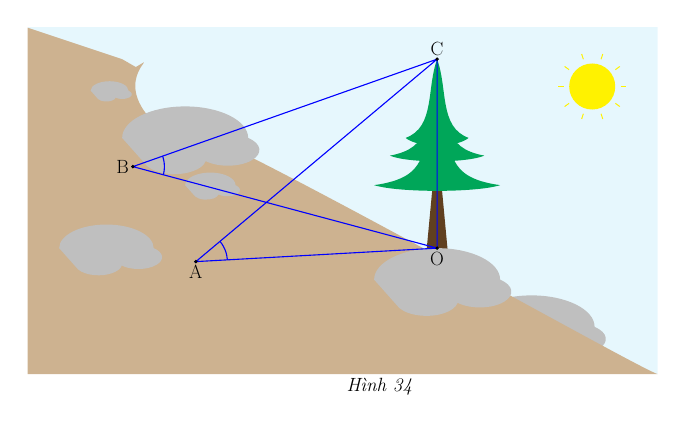
\begin{tikzpicture}[scale=0.4,transform shape,font=\LARGE]
			\draw[draw=none] (0,0)rectangle(20,11);
			\node[below right] at (current bounding box.south) {\textit{Hình 34}};
			\clip (0,0)rectangle(20,11);
			\fill[cyan!10](0,0)rectangle(27,15);
			\tikzset{Icon-mattroi/.pic={
					\def\r{0.35}
					\fill[opacity=1](0,0)circle(\r);
					\draw[line width=2*\r pt](0,0)circle(\r);
					\foreach \g in{1,...,10}{
						\draw[line width=\r pt](\g*36:1.2*\r)++(\g*36:0.1*\r)--++(\g*36:\r*0.25);
					}
			}}
			\tikzset{Doi-Oxyz/.pic={
					\fill[brown!90!teal!60](0,0)--(0,11)--(3,10)--++(-30:0.5)..controls++(-150:-1)and++(135:2)..(4,8)--++(20:0.25)..controls++(60:0.6) and++(160:1)..(20,0)--cycle;
			}}
			\tikzset{da/.pic={
					\fill[gray!50!white](0,0)arc(180:0: 2 and 1)arc(50:-135: 1 and 0.5)arc(-10:-150: 1 and 0.5);
			}}
			\tikzset{cay/.pic={
					\fill[brown!50!black](-0.75,-8)--(0.75,-8)--(0,0)--cycle;
					\fill[green!30!teal][xscale=2,yscale=0.75,shift={(0,-4)}](-2,0)..controls++(-40:1) and++(-140:1)..(2,0)..controls++(160:2)and++(-70:2)..(0,5)..controls++(-110:2)and++(20:2)..(-2,0);
					\fill[green!30!teal][xscale=1.5,yscale=0.75,shift={(0,-1.5)}](-2,0)..controls++(-40:1) and++(-140:1)..(2,0)..controls++(160:2)and++(-70:2)..(0,5)..controls++(-110:2)and++(20:2)..(-2,0);
					\fill[green!30!teal](-2,0)..controls++(-40:1) and++(-140:1)..(2,0)..controls++(160:2)and++(-70:2)..(0,5)..controls++(-110:2)and++(20:2)..(-2,0);
			}}
			\path(14,1.5)pic{da};
			\path(0,0)pic{Doi-Oxyz}(13,7.5)pic[scale=0.5]{cay};
			\foreach \x/\y/\sca in {1/4/0.75,11/3/1,5/6/0.4,3/7.5/1,2/9/0.3}
			\path(\x,\y)pic[scale=\sca]{da};
			\draw[blue](13,10)coordinate(C)--++(220:10)coordinate(A)--(13,4)coordinate(O)--cycle (O)--++(165:10)coordinate(B)--(C);
			\foreach \d in{O,A,B,C}
			\draw[fill=blue](\d)circle(1pt);
			\begin{scope}
				\clip(O)--(A)--(C)--cycle;
				\draw[blue](A)circle(1 cm);
			\end{scope}
			\begin{scope}
				\clip(O)--(B)--(C)--cycle;
				\draw[blue](B)circle(1 cm);
			\end{scope}
			\path(O)node[below]{O}(A)node[below]{A}(B)node[left]{B}(C)node[above]{C}(C)++(-10:5)pic[yellow,scale=2]{Icon-mattroi};
		\end{tikzpicture}
	}
\noindent Tính tổng số đó các góc tạo bởi mỗi dây neo và mặt phẳng sườn núi (làm tròn kết quả đến hàng đơn vị của độ).
\shortans{$92$}
	\loigiai{
	Ta có $\overrightarrow{O A}=(3 ;-4 ; 2), \overrightarrow{O B}=(-5 ;-2 ; 1)$ nên
			$$
			\left[\overrightarrow{OA}, \overrightarrow{O B}\right]=\left(\left|\begin{array}{ll}
				-4 & 2 \\
				-2 & 1
			\end{array}\right| ;\left|\begin{array}{cc}
				2 & 3 \\
				1 & -5
			\end{array}\right| ; \left| \begin{array}{cc}
				3 & -4 \\
				-5 & -2
			\end{array}\right|\right)=(0 ;-13 ;-26).
			$$
			Vì thế, véc-tơ $\overrightarrow{n}=(0 ; 1 ; 2)$ là một véc-tơ pháp tuyến của mặt phẳng $(O A B)$.\\
			Mặt khác, do $\overrightarrow{C A}=(3 ;-4 ;-3)$, $\overrightarrow{B C}=(5 ; 2 ; 4)$ nên ta có
			\[\sin (C A,(O A B))=|\cos (\overrightarrow{CA}, \overrightarrow{n})|=\dfrac{|\overrightarrow{C A} \cdot \overrightarrow{n}|}{|\overrightarrow{C A}| \cdot|\overrightarrow{n}|}=\dfrac{|3 \cdot 0+(-4) \cdot 1+(-3) \cdot 2|}{\sqrt{34} \cdot \sqrt{5}}=\dfrac{10}{\sqrt{170}}.\]
			Suy ra $(C A,(O A B)) \approx 50^{\circ}$. Vậy góc tạo bởi dây neo $C A$ và mặt phẳng sườn núi là khoảng $50^{\circ}$.\\
			Lại có
			$$
			\sin (B C,(O A B))=|\cos (\overrightarrow{B C}, \overrightarrow{n})|=\dfrac{|\overrightarrow{B C} \cdot \overrightarrow{n}|}{|\overrightarrow{B C}| \cdot|\overrightarrow{n}|}=\dfrac{|5 \cdot 0+2 \cdot 1+4 \cdot 2|}{3 \sqrt{5} \cdot \sqrt{5}}=\dfrac{2}{3},
			$$
			suy ra $(B C,(O A B)) \approx 42^{\circ}$. \\
			Vậy góc tạo bởi dây neo $B C$ và mặt phẳng sườn núi là khoảng $42^{\circ}$.\\
			Vậy tổng số đo $2$ góc là $92^\circ$.
	}
\end{ex}
\begin{ex}%[Nguyễn Tuấn, dự án sáng tác đề 12 theo chủ đề]%[2H5V2-7]
\immini{	Trong không gian với hệ tọa độ $Oxyz$, cho hình chóp $S.ABCD$ có các đỉnh lần lượt là $S\left(0;0;\dfrac{a\sqrt{3}}{2}\right)$, $A\left(\dfrac{a}{2};0;0\right)$, $B\left(-\dfrac{a}{2};0;0\right)$, $C\left(-\dfrac{a}{2};a;0\right)$, $D\left(\dfrac{a}{2};a;0\right)$ với $a>0$. Tính góc giữa đường thẳng $SD$ và mặt phẳng $(SAC)$ (làm tròn kết quả đến hàng đơn vị của độ).
	\shortans{$28$}
}{\begin{tikzpicture}[scale=0.7, font=\footnotesize,line join=round, line cap=round, >=stealth]
			\coordinate (B) at (0,0);
			\coordinate (A) at (-2,-2);
			\coordinate (J) at ($(A)!0.5!(B)$);
			\coordinate (x) at ($(B)!1.2!(A)$);
			\coordinate (C) at (5,0);
			\coordinate (D) at ($(A)+(C)-(B)$);
			\coordinate (I) at ($(C)!0.5!(D)$);
			\coordinate (y) at ($(J)!1.2!(I)$);
			\coordinate (S) at ($(J)+(0,4)$);
			\coordinate (z) at ($(J)!1.2!(S)$);
			\draw[dashed] (S)--(J)--(I);
			\draw[->](S)--(z) node[above]{$z$};
			\draw[->](I)--(y) node[below]{$y$};
			\draw[->](A)--(x) node[below,left]{$x$};
			\draw (S)--(C)--(D)--(A)--(S)--(D);
			\draw[dashed,thin] (C)--(B)--(A)--(D) (S)--(B);
			\draw (J) node[left]{$O$};
			\foreach \i/\g in {S/180,A/-90,B/-90,C/-90,D/-90}{\draw[fill=black](\i) circle (1.5pt) ($(\i)+(\g:3mm)$) node[scale=1]{$\i$};}
	\end{tikzpicture}}
	\loigiai{
		 Ta có $\overrightarrow{SA}=\left(\dfrac{a}{2};0;-\dfrac{\sqrt{3}}{2}\right)$, $\overrightarrow{SC}=\left(-\dfrac{a}{2};a;-\dfrac{a\sqrt{3}}{2}\right)$, 	$\overrightarrow{SD}=\left(\dfrac{a}{2};a;-\dfrac{\sqrt{3}}{2}\right)$.\\
			$\left[\overrightarrow{SA};\overrightarrow{SC}\right]=\left(\dfrac{a^2\sqrt{3}}{2};\dfrac{a^2\sqrt{3}}{2};\dfrac{a^2}{2}\right)=\dfrac{a^2}{2}\cdot \overrightarrow{n}$, với $\overrightarrow{n}=(\sqrt{3};\sqrt{3};1)$.\\
			Ta có\\
			$\sin(SD,(SAC))=\dfrac{|\overrightarrow{n}\cdot\overrightarrow{SD}|}{|\overrightarrow{n}|\cdot|\overrightarrow{SD}|}=\dfrac{\left|\dfrac{a\sqrt{3}}{2}+a\sqrt{3}-\dfrac{a\sqrt{3}}{2}\right|}{\sqrt{(\sqrt{3})^2+(\sqrt{3})^2+1^2}\cdot\sqrt{\left(\dfrac{a}{2}\right)^2+a^2+\left(\dfrac{-a\sqrt{3}}{2}\right)^2}}=\dfrac{\sqrt{42}}{4}$.\\
			Suy ra $(SD,(SAC))\approx 28^{\circ}$.
	}
\end{ex}
\begin{ex}%[Nguyễn Tuấn, dự án sáng tác đề 12 theo chủ đề]%[2H5V2-7]
	\immini
	{
		Để chuẩn bị cho chuyến đi dã ngoại, nhóm bạn Đức thiết kế lều cắm trại dạng hình chóp tứ giác đều có đáy là hình vuông cạnh $4$m. Theo bản vẽ thiết kế thì góc giữa hai mặt bên của lều bằng $60^{\circ}$. Bằng phương pháp tọa độ, hãy tính chiều cao của lều này (đơn vị: mét).
		\shortans{$2$}
	}
	{
		\begin{tikzpicture}[>=stealth,line join=round,line cap=round,font=\footnotesize,scale=1]
			\def \cao{3};
			\def \x{3};
			\coordinate (D) at (0,0);
			\coordinate (C) at (1,.8);
			\coordinate (A) at (\x,0);
			\coordinate (B) at ($(A)-(D)+(C)$);
			\coordinate (O) at ($(C)!.5!(A)$);
			\coordinate (S) at ($(O)+(90:\cao)$);
			\coordinate (X) at (intersection of S--O and  D--A);
			\draw (D)--(A)--(B)--(S)--cycle (S)--(A);
			\draw[dashed] (C)--(B) (S)--(C)--(D);
			\draw[dashed,red] (A)--($(A)!1.2!(C)$) (D)--(B) (S)--(X);
			\draw[->,red] (A)--($(O)!1.6!(A)$) node[right]{$x$};
			\draw[->,red] (B)--($(O)!1.4!(B)$) node[above]{$y$};
			\draw[->,red] (S)--($(O)!1.3!(S)$) node[left]{$z$};
			\draw[red] (X)--++(-90:0.7) (D)--($(O)!1.3!(D)$);
			\foreach \diem/\goc in {C/45,D/-90,A/-90,B/-30,S/45,O/-130} \fill[black](\diem) circle (1pt) ($(\diem)+(\goc:3mm)$) node{$\diem$};
		\end{tikzpicture}
	}
	\loigiai{
		Ta có $AC=BD=\sqrt{AD^2+AB^2}=\sqrt{4^2+4^2}=4\sqrt{2}$.\\
		Chọn hệ trục tọa độ $Oxyz$ với gốc tọa độ $O$ là giao điểm của hai đường chéo $AC$ và $BD$ như hình vẽ.\\
		Gọi $z$ là chiều cao của lều.\\
		Ta có $O(0;0;0)$, $A(2\sqrt{2};0;0)$, $B(0;2\sqrt{2};0)$, $C(-2\sqrt{2};0;0)$, $D(0;-2\sqrt{2};0),S(0;0;z)$, với $z>0$.\\
		Ta có $\overrightarrow{AD}=(-2\sqrt{2};-2\sqrt{2};0),\overrightarrow{AB}=(-2\sqrt{2};2\sqrt{2};0),\overrightarrow{AS}=(-2\sqrt{2};0;z)$.\\
		Véc-tơ pháp tuyến của $(SAD)$ là $\overrightarrow{n}_1=\left[\overrightarrow{AD},\overrightarrow{AS}\right]=(-2z\sqrt{2};2z\sqrt{2};-8)$.\\
		Véc-tơ pháp tuyến của $(SAB)$ là $\overrightarrow{n}_2=\left[\overrightarrow{AB},\overrightarrow{AS}\right]=(2z\sqrt{2};2z\sqrt{2};8)$.\\
		Ta có
		\begin{eqnarray*}
			\cos((SAD),(SAB))&=&\dfrac{|\overrightarrow{n}_1\cdot \overrightarrow{n}_2|}{|\overrightarrow{n}_1|\cdot |\overrightarrow{n}_2|}\\
			&=&\dfrac{|-2z\sqrt{2}\cdot 2z\sqrt{2}+2z\sqrt{2}\cdot 2z\sqrt{2}+8\cdot(-8)|}{\sqrt{(-2z\sqrt{2})^2+(2z\sqrt{2})^2+(-8)^2}\cdot \sqrt{(2z\sqrt{2})^2+(2z\sqrt{2})^2+8^2}}\\
			&=&\dfrac{64}{16z^2+64}.
		\end{eqnarray*}
		Vì góc giữa hai mặt bên bằng $60^{\circ}$ nên góc giữa hai mặt phẳng $(SAD)$ và $(SAB)$ bằng $60^{\circ}$.\\
		Do đó
		$$\cos 60^{\circ}=\dfrac{64}{16z^2+64} \Leftrightarrow \dfrac{1}{2}=\dfrac{64}{16z^2+64}\Leftrightarrow 16z^2+64=128\Leftrightarrow \hoac{&z=2\\&z=-2}$$
		Vì $z>0$ nên ta có $S(0;0;2)$.\\
		Vậy chiều cao của lều là $2$ m.
	}
\end{ex}
\Closesolutionfile{ans}
\indapan{6}{ans/ans-2-B16-De2-KQ}